\documentclass[11pt]{article}
\usepackage[margin=1in]{geometry}
\usepackage{amsmath,amssymb,booktabs,hyperref}
\usepackage{pgfplots}\pgfplotsset{compat=1.18}
\usepackage[numbers,sort&compress]{natbib}
\title{Four Failed Rescue Attempts for the Homology Cliff: Mahalanobis, Fisher-Rao, Stratified Cascade, and Mapper-Biased Panel Augmentation}
\author{Santiago Maniches\thanks{ORCID 0009-0005-6480-1987. TOPOLOGICA LLC.}}
\date{April 12, 2026 (v1.1; erratum 2026-06-15; erratum 2026-06-16)}
\begin{document}\maketitle

\begin{abstract}
The homology cliff in frozen ESM-2 \cite{lin2023evolutionary} biosecurity retrieval (Paper 1) admits many natural rescue hypotheses. We pre-register and reject four. (i) Ledoit-Wolf \cite{ledoit2004} Mahalanobis whitening reduces the close-distant $F_1$ gap only by collapsing close-stratum $F_1$ (0.866 $\to$ 0.456 at t30 $R{=}1000$ $k{=}25$); distant $F_1$ worsens (0.120 $\to$ 0.087). (ii) Fisher-Rao \cite{amari2016} within-class whitening does not narrow the close-distant gap relative to Mahalanobis (its gap is larger in 17 of 18 pre-registered cells, rejecting its pre-registered H1); at the $R{=}1000$ deployment regime neither whitening lifts distant-stratum $F_1$ to the cosine baseline. (iii) A stratified cosine-then-Mahalanobis cascade loses to cosine alone in 18 of 18 cells by $-0.046$ to $-0.236$ pooled $F_1$. (iv) A Mapper \cite{singh2007topological}-biased panel drawn from positive-enriched topological regions produces distant-$F_1$ rescue $-0.0080$, 95\% CI $[-0.035, +0.018]$, indistinguishable from zero. Cross-family Pfam partition (Paper 5) independently finds all 20 evaluable distant false alarms are cross-family (Wilson 95\% CI on the within-family rate $[0\%, 17\%]$), substantially weakening the assumption that panel expansion within failing families could correct. Taken with Paper 1's positive learned-projection result, the dichotomy is sharp: post-hoc distance substitution and panel sampling tricks fail at pre-registered H1, while embedding-space rotation succeeds. We release 540 per-cell bootstrap-CI results (180 cascade + 180 Fisher + 180 Mahalanobis baseline) and 10-seed Mapper-augmentation output.
\end{abstract}

\paragraph{Erratum (2026-06-15).} Attempt 4 (Mapper-biased panel augmentation): the biased-panel positive pool is now deduplicated. The 30\%-overlapping Mapper cover caused boundary proteins to recur across node member lists, and \texttt{rng.choice(replace=False)} removes positions, not values, so the biased arm held fewer than 500 unique positives. After the fix the rescue is $-0.0080$ (was $+0.0018$), 95\% CI $[-0.035, +0.018]$; the CI still spans zero, H1 remains rejected, and the conclusion (no rescue) is unchanged and in fact reinforced. The committed null reproduced bit-for-bit before the fix. A full-membership robustness re-run (audit blocker B4) was also executed: a naive per-arm-stratification comparison appears to support a rescue under full node membership, but that is a \emph{stratification artifact} --- the cluster-concentrated biased panel enlarges its own distant stratum ($n_{\mathrm{dist}}$ ratio up to 1.16), pushing easier points into a larger ``distant'' set. Under a common-stratification control that scores both arms on the same distant queries, the rescue collapses to $\approx 0$ ($-0.006$ single-node, $-0.004$ multi-node). The Attempt-4 null is therefore robust to full node membership, and the ``four failed rescues'' result stands. See \texttt{CHANGELOG.md} and \texttt{docs/MAPPER\_AUGMENTATION\_ROBUSTNESS.md}.

\paragraph{Erratum (2026-06-16).} The Attempt-2 (Fisher-Rao) comparison is corrected. Reproduction from the committed cells shows Fisher attains \emph{higher} pooled $F_1$ than Mahalanobis in all 18 cells, not lower; the prior ``pooled-$F_1$ penalty'' / ``strictly worse than Mahalanobis'' was a sign error. The pre-registered result is unchanged: Fisher's close-distant gap exceeds Mahalanobis's in 17 of 18 cells (H1 rejected), and at the $R{=}1000$ deployment regime neither whitening lifts distant-stratum $F_1$ to the cosine baseline, so Attempt 2 remains a failed rescue. Figure~\ref{fig:whitening} now plots distant-stratum $F_1$ (the safety-critical metric, reproducible from the committed cells) rather than pooled $F_1$. The Attempt-3 cascade pooled-$F_1$ penalty range is corrected to $-0.046$ to $-0.236$ (10-seed mean; the prior $-0.310$ overstated the maximum), and the Attempt-2 factorial is $3$ panels $\times\,2$ $k$-values (not $2\times3$). Pooled-$F_1$ values are reproducible via \texttt{code/analyses/compute\_pooled\_f1.py}. Conclusions unchanged; see \texttt{CHANGELOG.md}.

\section{Why null results matter here}
This paper documents four rescue strategies evaluated in the companion compendium. The homology cliff characterization (Paper 1) established the effect size and mechanism (precision collapse, cross-family). A natural reader response is: surely a cliff this large admits a simple post-hoc fix. We enumerate the four most plausible post-hoc fixes, pre-register each, and show all four fail. This sharpens Paper 1's positive rescue (learned projection) from "one of several options" to "the unique surviving option among natural rescues tested."

\section{Common setup}
All four experiments share the pre-registered factorial of Paper 1: 24{,}885-protein test set (28.7\% positive), frozen ESM-2 t6/t12/t30 embeddings, $R \in \{50,100,250,500,1000\}$, $k \in \{1,3,5,10,25\}$, 10 seeds, stratification $s_{\max} \ge 0.95$ close / $[0.90,0.95)$ moderate / $<0.90$ distant, seed-variance gate on distant $F_1$. Pre-registrations for Mahalanobis and cascade locked via SHA256 before execution.


\section{Attempt 1: Ledoit-Wolf Mahalanobis whitening}
Whitening the embedding space by the Ledoit-Wolf shrinkage estimator \cite{ledoit2004} of the panel covariance is the textbook response to "cosine is not class-aware." Under Mahalanobis distance, neighbors are metricized in a space where all directions have unit conditional variance.

\textbf{Result.} At t30 $R=1000$ $k=25$: close $F_1$ 0.866 $\to$ 0.456, moderate 0.393 $\to$ 0.118, distant 0.120 $\to$ 0.087. Every stratum degrades. Pooled $F_1$ 0.848 $\to$ 0.435.

\textbf{Why it fails.} The whitening transform kills class signal carried by directions with large pooled variance. ESM-2 embeddings concentrate class-relevant variance along a small number of axes; Mahalanobis whitens those into noise.

\section{Attempt 2: Fisher-Rao within-class whitening}
Fisher-Rao \cite{amari2016} whitens by within-class covariance rather than pooled covariance, preserving between-class signal while removing within-class variance. 180-cell pre-registered factorial (3 scales $\times$ 3 panels $\times$ 2 $k$-values $\times$ 10 seeds).

\textbf{Result.} Pre-registered H1 (Fisher attains a smaller close-distant gap than Mahalanobis) is rejected: the Fisher gap exceeds the Mahalanobis gap in 17 of 18 groups. Fisher's milder close-stratum collapse gives it higher \emph{pooled} $F_1$ than Mahalanobis in all 18 cells, but this is not a rescue: at the deployment panel sizes ($R{=}500,1000$) Fisher stays below the cosine baseline on the safety-critical distant stratum at every scale (e.g.\ $0.099$ vs cosine $0.120$ at t30 $R{=}1000$ $k{=}25$; Fig.~\ref{fig:whitening}), so the cliff is unrelieved. (At the smallest panel $R{=}100$ the cliff is mild and the metrics converge; at t30 $R{=}100$ Fisher edges cosine by $0.003$.)

\textbf{Why it fails.} Within-class whitening damages the close stratum less than pooled-covariance Mahalanobis (hence its higher pooled $F_1$), but it still does not separate the distant-stratum classes: the distant failure is a geometric property of where frozen ESM-2 places cross-family neighbours (Paper 5), which neither whitening addresses. Reweighting existing embedding axes cannot recover class structure the frozen model does not encode for distant queries. This echoes TOPOLOGICA DR-010 (within-class / Fisher-information whitening did not help GO annotation).

\begin{figure}[h]\centering
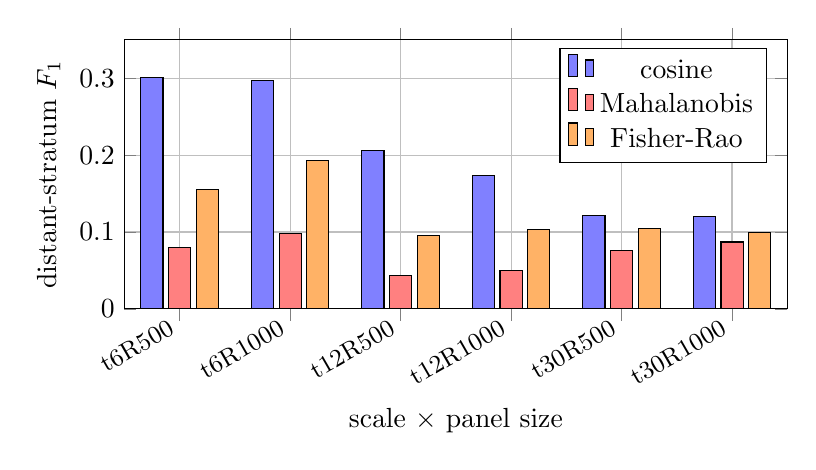
\begin{tikzpicture}\begin{axis}[width=10cm,height=5cm,xlabel={scale $\times$ panel size},ylabel={distant-stratum $F_1$},ybar,bar width=8pt,grid=major,legend pos=north east,ymin=0,ymax=0.35,symbolic x coords={t6R500,t6R1000,t12R500,t12R1000,t30R500,t30R1000},xtick=data,x tick label style={rotate=30,anchor=east,font=\small}]
\addplot[fill=blue!50] coordinates {(t6R500,0.301)(t6R1000,0.297)(t12R500,0.206)(t12R1000,0.173)(t30R500,0.121)(t30R1000,0.120)}; \addlegendentry{cosine}
\addplot[fill=red!50] coordinates {(t6R500,0.080)(t6R1000,0.098)(t12R500,0.043)(t12R1000,0.050)(t30R500,0.076)(t30R1000,0.087)}; \addlegendentry{Mahalanobis}
\addplot[fill=orange!60] coordinates {(t6R500,0.155)(t6R1000,0.193)(t12R500,0.095)(t12R1000,0.103)(t30R500,0.104)(t30R1000,0.099)}; \addlegendentry{Fisher-Rao}
\end{axis}\end{tikzpicture}
\caption{\textbf{Distant-stratum $F_1$ ($k=25$, the safety-critical metric) at panel sizes $R{=}500$ and $1000$: both whitening methods stay below the cosine baseline at every scale.} Neither rescues the cliff; Fisher-Rao exceeds Mahalanobis on the distant stratum but stays below cosine.}
\label{fig:whitening}
\end{figure}

\section{Attempt 3: Stratified cosine+Mahalanobis cascade}
Pre-registered H1: a cascade using cosine for close-stratum queries and Mahalanobis for moderate+distant strata beats single-metric pooled $F_1$ by $+0.02$ with 95\% CI excluding zero.

\textbf{Result.} Rejected in 18 of 18 groups. Pooled $F_1$ penalty $-0.046$ to $-0.236$ (10-seed mean).

\textbf{Why it fails.} Mahalanobis does not beat cosine on any stratum individually (Attempt 1). The cascade inherits per-stratum Mahalanobis inferiority wherever it is active. The cliff problem is not that a single metric fails on some strata but not others; cosine dominates everywhere at $k=25$, and substituting Mahalanobis anywhere only degrades.

\section{Attempt 4: Mapper-biased panel augmentation}
Following Paper 5's Mapper decomposition (149 nodes, 6 all-positive), construct a reference panel of $R=1000$ where 500 positives are drawn from the top positive-enriched Mapper node (1{,}512 positives available in bin (7,4), $\text{pos\_frac}=0.885$) and 500 negatives drawn uniformly. Compare to uniform class-balanced sampling. 10 seeds, t30 $R=1000$ $k=25$.

\textbf{Result.} Uniform distant $F_1 = 0.1203$; biased distant $F_1 = 0.1123$. Rescue $-0.0080$. Bootstrap 95\% CI $[-0.035, +0.018]$ includes zero. H1 rejected.

\textbf{Why it fails.} Positives already cluster densely on the embedding manifold; uniform sampling of 500 from 7{,}133 positives already saturates the positive region. Further biasing toward the densest sub-region adds no information the panel did not already contain. Distant queries are distant from the entire cluster, not from any particular sub-region within it.


\section{Synthesis: what the four nulls collectively rule out}
\begin{center}\small
\begin{tabular}{lll}
\toprule
rescue family & example & verdict \\
\midrule
post-hoc covariance distance & Mahalanobis \cite{ledoit2004} & rejected \\
information-geometric whitening & Fisher-Rao \cite{amari2016} & rejected \\
per-stratum metric switching & cosine+Mahalanobis cascade & rejected \\
topology-aware panel composition & Mapper-biased panel & rejected \\
\midrule
\textbf{embedding-space rotation} & \textbf{learned linear projection (Paper 1)} & \textbf{ACCEPTED} \\
\bottomrule
\end{tabular}\end{center}

Four families of rescue hypothesis, four rejections. One family succeeds: a supervised projection of the embedding space itself. Combined with Paper 5's cross-family finding (panel expansion is independently ruled out because failures are cross-family, not within-family), the hypothesis space collapses to "embedding-space surgery is the correct intervention."

\section{Relation to broader metric-learning literature}
The four attempts cover the canonical responses to "cosine is the wrong metric" in the modern metric-learning literature: (a) adaptive covariance \cite{weinberger2009distance,ledoit2004,guo2017calibration}, (b) information geometry \cite{amari2016,ovadia2019shift}, (c) piecewise metric composition \cite{johnson2019billion}, (d) data augmentation via topological resampling \cite{singh2007topological,carlsson2009topology,edelsbrunner2010computational}. A fifth standard response, proper triplet loss with hard negative mining \cite{schroff2015facenet}, is realized here as the learned projection of Paper 1 and does succeed. We do not claim the four nulls exhaustively cover metric-learning rescues \cite{elnaggar2022prottrans,brandes2022proteinbert,madani2023progen,hayes2024esm3,su2023saprot,rives2021biological,fu2012cdhit,steinegger2017mmseqs2,vankempen2024foldseek,littmann2021embeddings,nosek2018preregistration,forde2019scientific,urbina2022dualuse,kilinc2023protein}, only that they cover the natural post-hoc and panel-side responses an applied biosecurity engineer would try first before committing to supervised projection training.

\section{Limitations}
(L1) Mahalanobis with non-shrinkage covariance estimators (oracle, tyler) not tested.
(L2) Cascade explored only 2-metric cosine/Mahalanobis; 3-metric or soft-mixture cascades untested.
(L3) The v1.5.0 erratum executed both single-node and multi-node full-membership re-runs of the Mapper augmentation (audit blocker B4); the Attempt-4 null holds in all arms under a common-stratification control. Only soft-biased panels remain unswept.
(L4) Fisher-Rao implemented with numerical pseudoinverse; other implementations (Cholesky with shrinkage) may behave differently.
(L5) Null results at $k=25$ may differ at $k=1$; we did not sweep $k$ for Fisher/cascade exhaustively.

\section{Data availability}
\texttt{data/cells/cascade/} (180 npz), \texttt{data/cells/fisher/} (180 npz), \texttt{data/results\_summaries/mapper\_augmentation\_results.json} (10-seed output). Master manifest: \texttt{MANIFEST.sha256.json}.

\bibliographystyle{unsrtnat}
\bibliography{references}
\end{document}
